\documentclass{llncs}
\usepackage{algorithm}
\usepackage{algpseudocode}
\usepackage{fixltx2e}
\usepackage{subcaption}
\captionsetup{compatibility=false}
\usepackage{amsmath}
\usepackage{mathtools}
\usepackage{tikz}
\usetikzlibrary{trees}
\usetikzlibrary{positioning}
\usetikzlibrary{plotmarks}

\algnewcommand{\IIf}[1]{\State\algorithmicif\ #1\ \algorithmicthen}
\algnewcommand{\EndIIf}{}
\algnewcommand{\IfElse}[3]{\algorithmicif\ #1\ \algorithmicthen\ #2\ \algorithmicelse\ #3}
\algnewcommand{\EndIfElse}{}
\MakeRobust{\Call}
\newcommand{\True}{\texttt{true}}
\newcommand{\False}{\texttt{false}}
\newcommand{\II}{\mathcal{I}}
\newcommand{\textoverline}[1]{$\overline{\mbox{#1}}$}

\pagestyle{headings}

\begin{document}

\title{A SAT-Based Counterexample Guided Method for Unbounded Synthesis}

\author{Alexander Legg\inst{1} 
    \and Nina Narodytska\inst{2}
    \and Leonid Ryzhyk\inst{2}}

\institute{NICTA\thanks{NICTA is funded by the Australian Government as represented by the Department of Broadband,
    Communications and the Digital Economy and the Australian Research Council through the ICT
    Centre of Excellence program.} and UNSW \\
    \email{alexander.legg@nicta.com.au}
    \and Samsung Research America}

\maketitle

\sloppy

\begin{abstract}

    Reactive synthesis techniques based on constructing the winning region of
    the system have been shown to work well in many cases but suffer from state
    explosion in others.  A different approach, proposed recently, applies SAT
    solvers in a counterexample guided framework to solve the synthesis
    problem.  However, this method is limited to synthesising systems that
    execute for a bounded number of steps and is incomplete for synthesis with
    unbounded safety and reachability objectives.  We present an extension of
    this technique to unbounded synthesis.  Our method applies Craig
    interpolation to abstract game trees produced by counterexample guided
    search in order to construct a monotonic sequence of may-losing regions.
    Experimental results based on SYNTCOMP 2015 competition benchmarks show
    this to be a promising alternative that solves some previously intractable
    instances.

\end{abstract}

\section{Introduction}

Reactive systems are ubiquitous in real-world problems such as circuit design,
industrial automation, or device drivers. Automatic synthesis can provide a
\emph{correct by construction} controller for a reactive system from a
specification.  Reactive synthesis is formalised as a game between the \emph{controller} and
its \emph{environment}. In this work we focus on safety games, in which the
controller must prevent the environment from forcing the game into an error
state.

The reactive synthesis problem is EXPTIME-complete so
naive algorithms are infeasible on anything but simple systems.
% In this way the environment is equivalent to an existential search of
%the game and the controller is universal. Much of the complexity of reactive
%synthesis stems from managing the interactions of the alternating quantifiers
%on the state space of the game.
There are several techniques that aim to mitigate this complexity by
representing states and transitions of the system symbolically~\cite{Piterman_PS_06,bloem2014,morgenstern2013}. 
These techniques incrementally construct a symbolic representation of the set of 
discovered winning states of the game.  The downside of this approach is that 
keeping track of all discovered winning states can lead to a space explosion even
when using efficient symbolic representation such as BDDs or CNFs.

%Historically the most successful technique
%has been to use \emph{Binary Decision Diagrams}.  BDDs efficiently
%represent a relation on a set of game variables but in the worst case the
%representation may be exponential in the number of variables. As a result
%BDDs are not a one-size-fits-all solution for all reactive synthesis
%specifications.

%Advances in SAT solving technology has prompted research into its applicability
%to synthesis as an alternative to BDDs. One approach is to find sets of states
%in CNF \cite{bloem2014,morgenstern2013}. 

An alternative approach, proposed by Narodytska et al.~\cite{narodytska2014},
is to eschew states and focus on \emph{runs} of the game.  The method works by
exploring a subset of the concrete runs of the game and proving that these runs can be
generalised into a winning strategy on behalf of one of the players. In contrast to 
other existing synthesis methods, it does not store,
in either symbolic or explicit form, the set of winning states.
Instead, it uses counterexample guided backtracking search to identify a small subset
of runs that are sufficient to solve the game.

This method has been shown to outperform BDDs on certain classes of games; however it
suffers from an important limitation: it is only able to solve games with a bounded number
of rounds.  In case of safety games, this means proving that the controller 
can keep the game within the safe region for a bounded number of steps.  
This is insufficient in most practical situations that require unbounded realisability.

%Previous work has applied this idea to
%realisability of bounded games \cite{narodytska2014} by forming abstractions of
%the game and refining in a counterexample-guided framework.   

In this paper, we extend the method by Narodytska et al.~\cite{narodytska2014} to unbounded 
safety games.  To this end we enhance the method with computational learning: every time
the search algorithm discovers a new counterexample, the learning procedure analyzes the 
counterexample, extracting a subset of states winning for one of the players from it.  
The learning procedure ensures that reaching a fixed point in these sets is sufficient to establish 
unbounded realisability.
Our method can be seen as a hybrid between the counterexample guided algorithm
by Narodytska et al. and methods based on losing set computation: we use the
former to guide the search, while we rely on the latter to ensure convergence.

We evaluate our method on the benchmarks of the 2015 synthesis competition
(SYNTCOMP'15).  While our solver solves fewer total instances than competitors,
it solves the largest number of unique instances, i.e., instances that could not be solved by 
any other solver.  These results confirm that there exist classes of problems that are
hard for traditional synthesis techniques, but can be efficiently solved by our method.
While further performance improvements are clearly needed, in its current state the method 
can be used in a portfolio solver to increase the number of tractable instances.

Section 2 outlines the original bounded synthesis algorithm. In Section 3 we
describe and prove the correctness of our extension of the algorithm to
unbounded games. In the following sections we evaluate our methodology, and
compare our approach to other synthesis techniques.

\section{Background}

A \emph{safety game}, $G = \langle X, U, C, \delta, I, E \rangle$, is defined
over boolean state variables $X$, uncontrollable action variables $U$, and
controllable action variables $C$.  $I$ is the initial state of the game given
as a valuation of state variables.  $E(X)$ is the set of error states
represented by its characteristic formula.  The transition relation $\delta(X,
U, C, X')$ of the game is a boolean formula that relates current state and
action to the set of possible next states of the game.  We assume deterministic
games, where $\delta(x,u,c,x'_1) \land \delta(x,u,c,x'_2) \implies
(x'_1=x'_2)$.


At every round of the game, the \emph{environment} picks an uncontrollable
action, the \emph{controller} responds by choosing a controllable action and
the game transitions into a new state according to $\delta$.  A \emph{run} of a
game $(x_0, u_0, c_0), (x_1, u_1, c_1) \dots (x_n, u_n, c_n)$ is a chain of
state and action pairs s.t.\,$\delta(x_k, u_k, c_k, x_{k+1})$.  A run is
winning for the controller if $x_0 = I \land \forall i \in \{1..n\} (\lnot
E(x_i))$.  In a \emph{bounded game} with maximum bound $\kappa$ all runs are
restricted to length $\kappa$, whereas unbounded games consider runs of
infinite length.  Since we consider only deterministic games, a run is uniquely
described by a list of assignments to $U$ and $C$.

A \emph{controller strategy} $\pi^c : (2^X, 2^U) \to 2^C$ is a mapping of states and
uncontrollable inputs to controllable actions. A controller strategy is winning
in a bounded game of maximum bound $\kappa$ if all runs $(x_0, u_0, \pi^c(x_0,
u_0)), (x_1, u_1, \pi^c(x_1, u_1)) \dots$ $(x_n, u_n, \pi^c(x_n, u_n))$ are
winning.  Bounded \emph{realisability} is the problem of determining the
existence of such a strategy for a bounded game.

An \emph{environment strategy} $\pi^e : 2^X \to 2^U$ is a mapping of states to
uncontrollable actions. A bounded run is winning for the environment if $x_0 =
I \land \exists i \in \{1..n\} (E(x_i))$ and an environment strategy is winning
for a bounded game if all runs $(x_0, \pi^e(x_0), c_0), (x_1, \pi^e(x_1), c_1)
\dots (x_n, \pi^e(x_n), c_n)$ are winning for the environment.  Safety games
are zero sum, therefore the existence of a winning controller strategy implies
the nonexistence of a winning environment strategy and vice versa.

\subsection{Counterexample guided bounded synthesis}

We review the bounded synthesis algorithm by Narodytska et
al.~\cite{narodytska2014}, which is the main building block for our unbounded
algorithm.

First, we introduce a running example to assist the explanation. We consider a
simple arbiter system in which the environment requests for either 1 or 2
resources, and the controller may grant access to two resources. The controller
must ensure that the number of unhandled requests is not $\geq 3$.
Figure~\ref{fig:example} shows the variables (\ref{fig:examplevars}) and the
formulas for computing next-state variables (\ref{fig:exampletrans}) for this
example.

\begin{figure}
    \begin{subfigure}[t]{\textwidth}
        \centering
        \begin{tabular}{l | l | l}
            \textbf{Controllable} & \textbf{Uncontrollable} & \textbf{State} \\
            \hline
            \texttt{request = \{1, 2\}} & \texttt{grant0 = \{0, 1\}} & \texttt{resource0 = \{0, 1\}} \\
            & \texttt{grant1 = \{0, 1\}} & \texttt{resource1 = \{0, 1\}} \\
            & & \texttt{nrequests = \{0, 1, 2, 3\}} \\
        \end{tabular}
        \caption{Variables}
        \label{fig:examplevars}
    \end{subfigure}

    \begin{subfigure}[t]{\textwidth}
        \begin {align*}
            \texttt{resource0'} & \texttt{ = grant0;} \\
            \texttt{resource1'} & \texttt{ = grant1;} \\
            \texttt{nrequests'} & \texttt{ = (nrequests + request >= resource0 + resource1)} \\ 
                                & \texttt{ ? (nrequests + request - resource0 - resource1) : 0;}
        \end{align*}
        \caption{Transition Relation}
        \label{fig:exampletrans}
    \end{subfigure}
    \caption{Example}
    \label{fig:example}
\end{figure}


The bounded synthesis algorithm consists of two competing solvers, one for the
controller and one for the environment, that solve abstractions of the safety
game. Each solver builds a candidate strategy for its corresponding player
consisting of assignments to $2^C$ and $2^U$ respectively. 

The game abstraction is initially constructed from an opponent candidate
strategy. It is refined by counterexamples to the solver's own candidate
strategy that are formed when the opponent solves the abstract game
corresponding to that strategy. By abstracting the game in this way we
conceptually direct the solvers' search to consider opponent actions that may
lead to winning strategies.

An abstraction of the game restricts actions available to one of the players.
Specifically, we consider abstractions represented as trees of actions,
referred to as \emph{abstract game trees} (AGTs).  Figure~\ref{fig:agt} shows
an example abstract game tree restricting the environment (abstract game trees
restricting the controller are similar).  In the abstract game, the controller
can freely choose actions whilst the environment is required to pick actions
from the tree.  After reaching a leaf, the enivironment continues playing
unrestricted.  The tree in Figure~\ref{fig:agt} restricts the first and second
environment actions to \texttt{request=1}. It then reaches a leaf of the tree
and continues playing unrestricted. 

The root of the tree is annotated by the initial state $s$ of the abstract game
and the bound $k$ on the number of rounds.  We denote $\textsc{nodes}(T)$ the
set of all nodes of a tree $T$, $\textsc{leaves}(T)$ the subset of leaf nodes.
For edge $e$, $\textsc{action}(e)$ is the action that labels the edge, and for
node $n$, $\textsc{height}(k, n)$ is the distance from n to the last round of a
game bounded to $k$ rounds.  $\textsc{height}(k, T)$ is the height of the root
node of the tree.  For node $n$ of the tree, $\textsc{succ}(n)$ is the set of
pairs $\langle e, n' \rangle$ where $n'$ is a child node of $n$ and $e$ is the
edge connecting $n$ and $n'$.

\tikzset{every node/.style={solid}}
\tikzstyle{fixed}=[solid]
\tikzstyle{unfixed}=[dash pattern = on 2pt off 2pt]
\begin{figure}
    \centering
    \begin{subfigure}[t]{.25\textwidth}
        \centering
        \begin{tikzpicture}[dash pattern = on 2pt off 2pt, level distance = 10mm]
            \node [circle,draw] (root){}
                child {node [circle,draw] {}
                    child {node [circle,draw] {}
                        edge from parent [fixed] node [left] {\texttt{req=1}}
                    }
                    edge from parent [fixed] node [left] {\texttt{req=1}}
                }
%%%                child {node [circle,draw] {}
%%%                    edge from parent [fixed] node [right] {\texttt{gr=1}}
%%%                }
                node [above=4pt] {$\langle s, k \rangle$};
        \end{tikzpicture}
        \captionsetup{width=.8\textwidth}
        \caption{AGT}
        \label{fig:agt}
    \end{subfigure}%
    \begin{subfigure}[t]{.25\textwidth}
        \centering
        \begin{tikzpicture}[dash pattern = on 2pt off 2pt, level distance = 10mm]
            \node [circle,draw] (root){}
                child {node [circle,draw] {}
                    child {node [circle,draw] {}
                        node [left=4pt] {\texttt{gr0=1, gr1=0}}
                        edge from parent [fixed] node [left] {\texttt{req=1}}
                    }
                    node [left=4pt] {\texttt{gr0=0, gr1=1}}
                    edge from parent [fixed] node [left] {\texttt{req=1}}
                }
%%%                child {node [circle,draw] {}
%%%                    node [left=4pt] {\texttt{req=1}}
%%%                    edge from parent [fixed] node [right] {\texttt{gr=1}}
%%%                }
                node [left=4pt] {}
                node [above=4pt] {$\langle s, k \rangle$};
        \end{tikzpicture}
        \captionsetup{width=.8\textwidth}
        \caption{AGT with partial strategy}
        \label{fig:strategy}
    \end{subfigure}%
    \begin{subfigure}[t]{.25\textwidth}
        \centering
        \begin{tikzpicture}[dash pattern = on 2pt off 2pt, level distance = 10mm]
            \node [circle,draw] (root){}
                child {node [circle,draw] {}
                    child {node [circle,draw] {}
                        edge from parent [fixed] node [left] {\texttt{req=1}}
                    }
                    child {node [circle,draw] {}
                        edge from parent [fixed] node [right] {\texttt{req=2}}
                    }
                    edge from parent [fixed] node [left] {\texttt{req=1}}
                }
                node [above=4pt] {$\langle s, k \rangle$};
        \end{tikzpicture}
        \captionsetup{width=.8\textwidth}
        \caption{Refined AGT}
        \label{fig:refined}
    \end{subfigure}%
    \begin{subfigure}[t]{.25\textwidth}
        \centering
        \begin{tikzpicture}[scale=0.75,dash pattern = on 2pt off 2pt, level distance = 10mm]
            \node [circle,draw] (root){}
                child {node [circle,draw] {}
                    child {node [circle,draw] {}
                        child {node [circle,draw] {}
                            edge from parent [fixed] node [left] {$c$}
                        }
                        edge from parent [fixed] node [left] {$b$}
                    }
                    edge from parent [fixed] node [left] {$a$}
                }
                child {node [circle,draw] {}
                    child {node [circle,draw] {}
                        child {node [circle,draw] {}
                            edge from parent [fixed] node [left] {$f$}
                        }
                        edge from parent [fixed] node [right] {$e$}
                    }
                    edge from parent [fixed] node [right] {$d$}
                }
                node [above=4pt] {$\langle s, 3 \rangle$};
        \end{tikzpicture}
        \captionsetup{width=.8\textwidth}
        \caption{AGT extended to bound 3 with arbitrary controller actions}
        \label{fig:extended}
    \end{subfigure}
    \caption{Abstract game trees.}
    \label{fig:alltrees}
\end{figure}

Given an environment (controller) abstract game tree $T$ a \emph{partial
strategy} $Strat: \textsc{nodes}(T) \rightarrow C$ ($Strat: \textsc{nodes}(T)
\rightarrow U$) labels each node of the tree with the controller's
(environment's) action to be played in that node.   Given a partial strategy
$Strat$, we can map each leaf $l$ of the abstract game tree to $\langle
s',i'\rangle=\textsc{outcome}(\langle s, i\rangle, Strat, l)$ obtained by
playing all controllable and uncontrollable actions on the path from the root
to the leaf.  Figure~\ref{fig:strategy} shows an example partial strategy for
the controller.  The controller responds to the requests by first granting
access to \texttt{resource1}, then to \texttt{resource0} in the second round.

The bounded synthesis algorithm solves abstract game trees by invoking a SAT
solver to search for candidate partial strategies. Candidate strategies are
checked by a call to the opponent solver, which also refines the abstract
game tree. The refinements are then solved recursively.  The full procedure is
illustrated in Algorithm~\ref{alg:bounded}.

\begin{algorithm}[t]
    \begin{algorithmic}[1]
        \Function{solveAbstract}{$p, s, k, T$}
        \State $cand \gets $ \Call{findCandidate}{$p, s, k, T$} \Comment{Look for a candidate}
        \IIf{$k = 1$} \Return $cand$ \EndIIf \Comment{Reached the bound}
        \State $T' \gets T$
        \Loop
            \IIf{$cand = \texttt{NULL}$} \Return $\texttt{NULL}$ \EndIIf \Comment{No candidate: return with no solution}
            \State $\langle cex, l, u \rangle \gets $ \Call{verify}{$p, s, k, T, cand$} \Comment{Verify candidate}
            \IIf{$cex = \False$} \Return $cand$ \EndIIf \Comment{No counterexample: return candidate}
            \State $T' \gets $ \Call{append}{$T', l, u$} \Comment{Refine $T'$ with counterexample}
            \State $cand \gets $ \Call{solveAbstract}{$p, s, k, T'$} \Comment{Solve refined game tree}
        \EndLoop
        \EndFunction
        \algstore{b1}
    \end{algorithmic}

    \begin{algorithmic}
        \algrestore{b1}
        \Function{findCandidate}{$p, s, k, T$}
        \State $\hat{T} \gets $ \Call{extend}{$T$} \Comment{Extend the tree with unfixed actions}
            \State $f \gets $ \IfElse{$p = \texttt{cont}$}{\Call{treeFormula}{$k, \hat{T}$}}{\Call{\textoverline{treeFormula}}{$k, \hat{T}$}} \EndIfElse
            \State $sol \gets $ \Call{SAT}{$s(X_{\hat{T}}) \land f$}
            \If{$sol = \texttt{unsat}$} 
                \If{\texttt{unbounded}} \Comment{Active only in the unbounded solver}
                    %\State $\sigma \gets $ \Call{generalise}{$s$} \Comment{Expand $s$ to a set of states}
                    \State \IfElse{$p = \texttt{cont}$}{\Call{learn}{$s, \hat{T}$}}{\Call{\textoverline{learn}}{$s, \hat{T}$}} \EndIfElse
                \EndIf
                \State \Return $\texttt{NULL}$ \Comment{No candidate exists}
            \Else
                \State \Return $\{ \langle n, c \rangle | n \in $ \Call{nodes}{$T$} $, c = \Call{sol}{n} \}$ \Comment{Fix candidate moves in $T$}
            \EndIf
        \EndFunction
        \algstore{b2}
    \end{algorithmic}

    \begin{algorithmic}
        \algrestore{b2}
        \Function{verify}{$p, s, k, T, cand$}
            \For{$l \in leaves(gt)$}
            \State $\langle k', s'\rangle \gets $ \Call{outcome}{$s, k, cand, l$} \Comment{Get bound and state at leaf}
                \State $u \gets $ \Call{solveAbstract}{\Call{opponent}{$p$}, $s'$, $k'$, $\emptyset$} \Comment{Solve for the opponent}
                \IIf{$u \neq \texttt{NULL}$} \Return $\langle \True, l, u \rangle$ \EndIIf \Comment{Return counterexample}
            \EndFor
            \State \Return $\langle \False, \emptyset, \emptyset \rangle$
        \EndFunction
    \end{algorithmic}

    \caption{Bounded synthesis}
    \label{alg:bounded}
\end{algorithm}

The algorithm takes a concrete game $G$ with maximum bound $\kappa$ as an implicit
argument.  In addition, it takes a player $p$ (controller or environment),
state $s$, bound $k$ and an abstract game tree $T$ and returns a winning
partial strategy for $p$, if one exists.  The initial invocation of the
algorithm takes the initial state $I$, bound $\kappa$ and an empty abstract
game tree $\emptyset$.  Initially the solver is playing on behalf of the
environment since that player takes the first move in every game round.  The
empty game tree does not constrain opponent moves, hence solving such an
abstraction is equivalent to solving the original concrete game.

The algorithm is organised as a counterexample-guided abstraction refinement
(CEGAR) loop.  The first step of the algorithm uses the \textsc{findCandidate}
function, described below, to come up with a candidate partial strategy that is
winning when the opponent is restricted to $T$.  If it fails to find a
strategy, this means that no winning strategy exists against the opponent
playing its partial strategy represented by $T$.  If, on the other hand, a
candidate partial strategy is found, we need to verify if it is indeed winning
for the abstract game $T$.

The \textsc{verify} procedure searches for a \emph{spoiling} counterexample
strategy in each leaf of the candidate partial strategy by calling
\textsc{solveAbstract} for the opponent. The dual solver solves games on behalf
of the controller player.  

If the dual solver can find no spoiling strategy at any of the leaves, then the
candidate partial strategy is a winning one. Otherwise, \textsc{verify} returns
the move used by the opponent to defeat a leaf of the partial strategy, which
is appended to the corresponding node in $T$ in order to refine it in line~(9).
In our example, the controller's partial strategy in Figure~\ref{fig:strategy}
is defeated by the counterexample action \texttt{req=2}.
Figure~\ref{fig:refined} shows a refined AGT that includes this action.

We solve the refined game by recursively invoking \textsc{solveAbstract} on it.
If no partial winning strategy is found for the refined game then there is also
no partial winning strategy for the original abstract game, and the algorithm
returns a failure.  Otherwise, the partial strategy for the refined game is
\emph{projected} on the original abstract game by removing the leaves
introduced by refinements. The resulting partial strategy becomes a candidate
strategy to be verified at the next iteration of the loop. In the worst case
the loop terminates after all actions in the game are refined into the abstract
game.

The CEGAR loop depends on the ability to guess candidate partial strategies in
\textsc{findCandidate}. For this purpose we use the heuristic that a partial
strategy may be winning if each \textsc{outcome} of the strategy can be
extended to a run of the game that is winning for the current player.  Clearly,
if such a partial strategy does not exist then no winning partial strategy can
exist for the abstract game tree. We can formulate this heuristic as a SAT
query, which is constructed recursively by $\textsc{treeFormula}$ (for the
controller) or $\textsc{\textoverline{treeFormula}}$ (for the environment) in
Algorithm~\ref{alg:treeFormula}.

The tree is first extended to the maximum bound with edges that are labeled
with arbitrary opponent actions (Algorithm~\ref{alg:bounded}, line 14) as shown
in Figure~\ref{fig:extended}.  For each node in the tree, new SAT variables are
introduced corresponding to the state ($X_T$) and action ($U_T$ or $C_T$)
variables of that node. Additional variables for the opponent actions in the
edges of $T$ are introduced ($U_e$ or $C_e$) and set to $\textsc{action}(e)$.
The state and action variables of node $n$ are connected to successor nodes
$\textsc{succ}(n)$ by an encoding of the transition relation and constrained to
the winning condition of the player.

%%%Then copies of state and action variables are introduced for each node in the
%%%tree and opponent action variables for each edge $e$ are set to
%%%$\textsc{action}(e)$. 

%%%Candidates are discovered by passing a formulation of the abstract game tree to
%%%a SAT solver in $\textsc{findCandidate}$. This formula contains CNF encodings
%%%of all of the unrolled runs represented by the tree and the winning condition
%%%of the current player.  Runs are encoded by copying the transition relation for
%%%every step in the abstract game. When playing for the controller, the SAT
%%%solver searches for a satisfying assignment to the unfixed label variables in
%%%tree so that none of the runs reaches the error state. The environment
%%%formulation is satisfiable if any run does reach the error state.  The formula
%%%is constructed recursively from the root of a tree by $\textsc{treeFormula}$
%%%(see Algorithm~\ref{alg:treeFormula}).

%%%Since the game tree formulation is passed to a SAT solver, both controllable
%%%and uncontrollable unfixed labels will be existentially quantified. This means
%%%that the SAT solver will find any way to win the game while both players are
%%%cooperating. If no winning run exists in an abstract game even when the players
%%%are cooperating then there is no winning run when the opponent is playing
%%%adversarily. When a winning run is found, the actions chosen by the SAT solver
%%%are used to refine the game tree. This is advantageous for many synthesis
%%%problems where the game must be formalised as adversarial for correctness but
%%%the final implementation will cooperate with its environment in the real world.
%%%An example of such a system is a device driver that cooperates with the device
%%%and OS to provide the interface between the two.

\begin{algorithm}
    \caption{Tree formulas for Controller and Environment respectively}
    \label{alg:treeFormula}
    \begin{algorithmic}[1]
        \Function{treeFormula}{$k, T$}
        \If{$\Call{height}{k, T} = 0$}
        \State \Return{ $\lnot \Call{E}{X_{T}}$ }
        \Else
        \State \Return{$\lnot \Call{E}{X_{T}} \land$ \\
            $$\bigwedge_{\langle e, n \rangle \in \Call{succ}{T}}(\Call{$\delta$}{X_T, U_e, C_T, X_n} \land U_e = \Call{action}{e} \land \Call{treeFormula}{k, n})$$
        }
        \EndIf
        \EndFunction
        \algstore{tf1}
    \end{algorithmic}

    \begin{algorithmic}[1]
        \algrestore{tf1}
        \Function{\textoverline{treeFormula}}{$k, T$}
        \If{$\Call{height}{k, T} = 0$}
        \State \Return{\Call{E}{$X_{T}$}}
        \Else
        \State \Return{ $\Call{E}{X_{T}} \lor$ \\
        $$\bigvee_{\langle e, n \rangle \in \Call{succ}{T}}(\Call{$\delta$}{X_T, U_T, C_e, X_n} \land C_e = \Call{action}{e} \land \Call{\textoverline{treeFormula}}{k, n})$$ }
        \EndIf
        \EndFunction
    \end{algorithmic}
\end{algorithm}

\section{Unbounded Synthesis}

\label{sect:unbounded}

Bounded synthesis can be used to prove the existence of a winning strategy for
the environment on the unbounded game by providing a witness. For the
controller, the strongest claim that can be made is that the strategy is
winning as long as the game does not extend beyond the maximum bound.

It is possible to set a maximum bound such that all runs in the unbounded game will be
considered. The na\"ive approach is to use size of the state space as the bound
($2^{|X|}$) so that all states may be explored by the algorithm. A more nuanced
approach is to use the diameter of the game \cite{biere1999}, which is the
smallest number $d$ such that for any state $x$ there is a path of length $\leq
d$ to all other reachable states. However, the diameter is difficult to
estimate and can still lead to infeasibly long games.

We instead present an approach that iteratively solves games of increasing
bound while learning winning states from abstract games using interpolation. We
show that reaching a fixed point in learned states is sufficient for
completeness.

%%%\subsection{Extending Bounded Synthesis to Unbounded Games}


%%%During the CEGAR loop of the bounded algorithm, each of the competing solvers
%%%searches for satisfying assignments of labels to abstract game trees. When the
%%%abstract game is unsatisfiable this indicates that the states represented by
%%%nodes in the abstract game tree are losing for the current player. We extract
%%%these states from the game tree using interpolation.

%%%When executing the unbounded solver, lines 19 and 20 become active in the
%%%bounded solver. These lines call the learning procedures when the solver fails
%%%to find a candidate for an abstract game tree. The states symbolically
%%%represented by nodes in the tree are losing for whichever player could not find
%%%a winning candidate and can be extracted from the tree using interpolation.

%%%The states in an abstract game with no controller candidate are
%%%\emph{must-losing}. The environment can always force the game into the error
%%%states from these states.

%%%From abstractions with no environment candidate we record the complement of
%%%states in the tree as \emph{may-losing}. The environment cannot reach the error
%%%state in a number of steps equal to the distance to the bottom of the tree.

%%%We maintain a set of states for each rank up to the current bound. We maintain
%%%an invariant over these sets via careful construction so that they are
%%%monotonically increasing by rank. We also ensure that the environment is unable
%%%to force play from one set to the next. Due to these invariants, when two
%%%adjacent sets become equivalent we know that the algorithm has reached a fixed
%%%point and the controller is winning in the unbounded game (line 6).

\subsection{Learning States with Interpolants}

We extend the bounded synthesis algorithm to learn states losing for one of the
players from failed attempts to find candidate strategies.  The learning
procedure kicks in whenever \textsc{findCandidate} cannot find a candidate
strategy for an abstract game tree $T$ with initial state $s$ and bound $k$.
For the controller, this means the environment partial strategy represented by $T$
will always reach $E$ from $s$ no matter the assignments to $C$ variables (the
bound is irrelevant).  For the environment, the controller can avoid $E$ for $k$
rounds no matter the assignments to $U$ variables. Hence, we have established
that $s$ is a losing state either always (for the controller) or for bound $k$ (for
the environment. We can learn additional losing states from the tree via
interpolation.  This is achieved in lines~18--20 in
Algorithm~\ref{alg:bounded}, enabled in the unbounded version of the algorithm,
which invoke \textsc{learn} or \textsc{\textoverline{learn}} to learn
controller or environment losing states respectively
(Algorithm~\ref{alg:learn}).

\begin{figure}[t]
    \centering
    \begin{subfigure}[t]{.32\textwidth}
        \centering

        \begin{tikzpicture}[dash pattern = on 2pt off 2pt, level distance = 10mm]
            \node [circle,draw] (root){}
                child {node [circle,draw] {}
                    child {node [circle,draw,right=5pt] {}
                        edge from parent [fixed] node [left] {\texttt{gr0=1, gr1=0}}
                    }
                    child {node [circle,draw,left=5pt] {}
                        edge from parent [fixed] node [right] {\texttt{gr0=1, gr1=1}}
                    }
                    node [left=5pt] {$n$}
                    edge from parent [fixed] node [left] {\texttt{gr0=0, gr1=1}}
                }
                child {node [circle,draw] (n) {}
                    child {node [circle,draw] {}
                        edge from parent [fixed] node [right] {\texttt{gr0=1, gr1=1}}
                    }
                    edge from parent [fixed] node [right] {\texttt{gr0=1, gr1=1}}
                }
                node [above=4pt] {$\langle s, k \rangle$};
        \end{tikzpicture}
        \caption{A losing AGT $T$}
        \label{fig:interpolatetree}
    \end{subfigure}%
    \begin{subfigure}[t]{.32\textwidth}
        \centering
        \begin{tikzpicture}[dash pattern = on 2pt off 2pt, level distance = 10mm]
            \node [circle,draw] (root){}
                child {node [circle,draw] {}
                    node [left=5pt] {$n$}
                    edge from parent [fixed] node [left] {\texttt{gr0=1, gr1=0}}
                }
                child {node [circle,draw] (n) {}
                    child {node [circle,draw] {}
                        edge from parent [fixed] node [right] {\texttt{gr0=1, gr1=1}}
                    }
                    edge from parent [fixed] node [right] {\texttt{gr0=1, gr1=1}}
                }
                node [above=4pt] {$\langle s, k \rangle$};
        \end{tikzpicture}
        \caption{Tree slice $T_1$}
        \label{fig:treef1}
    \end{subfigure}%
    \begin{subfigure}[t]{.32\textwidth}
        \centering
        \begin{tikzpicture}[dash pattern = on 2pt off 2pt, level distance = 10mm]
            \node [circle,draw] {}
                child {node [circle,draw,right=5pt] {}
                    edge from parent [fixed] node [left] {\texttt{gr0=1, gr1=0}}
                }
                child {node [circle,draw,left=5pt] {}
                    edge from parent [fixed] node [right] {\texttt{gr0=1, gr1=1}}
                }
                node [left=5pt] {$n$};
        \end{tikzpicture}
        \caption{Tree slice $T_2$}
        \label{fig:treef2}
    \end{subfigure}
    \caption{Splitting of an abstract game tree by the learning procedure.}
\end{figure}

\begin{algorithm}[t]
    \begin{algorithmic}[1]
        \Require $s(X_T) \land $ \Call{treeFormula}{$k, T$} $\equiv \bot$
        \Require \emph{Must-invariant} holds
        \Ensure \emph{Must-invariant} holds
        \Ensure $s(X_T) \land B^M \not\equiv \bot$
        \Comment $s$ will be added to $B^M$
        \Function{learn}{$s, T$}
            \IIf{\Call{succ}{$T$} $= \emptyset$}
                \Return
            \EndIIf
            \State $n \gets $ non-leaf node with min height 
            \State $\langle T_1, T_2 \rangle \gets $ \Call{gtSplit}{$T, n$}
            \State $\mathcal{I} \gets $ \Call{interpolate}{$s(X_T) \land $ \Call{treeFormula}{$k, T_1$}, \Call{treeFormula}{$k, T_2$}}
            \State $B^M \gets B^M \lor \mathcal{I}$
            \State \Call{learn}{$s, T_1$}
        \EndFunction
        \algstore{learn}
    \end{algorithmic}
    
    \begin{algorithmic}[1]
        \algrestore{learn}
        \Require $s(X_T) \land $ \Call{\textoverline{treeFormula}}{$k, T$} $\equiv \bot$
        \Require \emph{May-invariant} holds
        \Ensure \emph{May-invariant} holds
        \Ensure $s(X_T) \land B^m[$\Call{height}{$k, T$}$] \equiv \bot$
        \Comment{$s$ will be removed from $B^m$}
        \Function{\textoverline{learn}}{$s, T$}
            \IIf{\Call{succ}{$T$} $= \emptyset$}
                \Return
            \EndIIf
            \State $n \gets $ non-leaf node with min height 
            \State $\langle T_1, T_2 \rangle \gets $ \Call{gtSplit}{$T, n$}
            \State $\mathcal{I} \gets $ \Call{interpolate}{$s(X_T) \land $ \Call{\textoverline{treeFormula}}{$k, T_1$}, \Call{\textoverline{treeFormula}}{$k, T_2$}}
            \For{$i = 1$ to \Call{height}{$k, n$}}
                \State $B^m[i] \gets B^m[i] \setminus \mathcal{I}$
            \EndFor
            \State \Call{\textoverline{learn}}{$s, T_1$}
        \EndFunction
    \end{algorithmic}
    \caption{Learning algorithms}
    \label{alg:learn}
\end{algorithm}

Consider the game tree $T$ in
Figure~\ref{fig:interpolatetree}, whose edges are labelled with environment
actions.  Assume that there does not exist a partial strategy for the controller
winning against this tree and that the \textsc{findCandidate} function could
not find a candidate strategy. We choose a non-leaf node $n$ of $T$ with
maximal depth, i.e., a node whose children are leafs
(Algorithm~\ref{alg:learn}, line~3). We then split the tree at $n$ such that
both slices $T_1$ and $T_2$ contain a copy of $n$ (line~4).
Figure~\ref{fig:treef1} shows $T_1$, which contains all of $T$ except $n$'s
children, and $T_2$ (Figure~\ref{fig:treef2}), which contains only $n$ and its
children.  There is no candidate strategy for $T$ so $s \land
\textsc{treeFormula}(k, T)$ is unsatisfiable.  By construction,
$\textsc{treeFormula}(k, T) \equiv \textsc{treeFormula}(k, T_1) \land
\textsc{treeFormula}(k, T_2)$ and hence $s \land \textsc{treeFormula}(k, T_1) \land
\textsc{treeFormula}(k, T_2)$ is also unsatisfiable. This enables the construction
of an \emph{interpolant} that captures losing states at node $n$.

Given two formulas $F_1$ and $F_2$ such that $F_1 \land F_2$ is unsatisfiable,
it is possible to construct a Craig interpolant~\cite{craig1957} $\mathcal{I}$
such that $F_1 \to \mathcal{I}$, $F_2 \land \mathcal{I}$ is unsatisfiable, and
$\mathcal{I}$ refers only to the intersection of variables in $F_1$ and $F_2$.
An interpolant can be constructed efficiently from a resolution proof of the
unsatisfiability of $F_1 \land F_2$~\cite{pudlak1997}.

We construct an interpolant with $F_1 = s(X_T) \land \textsc{treeFormula}(k, T_1)$
and $F_2 = \textsc{treeFormula}(k, T_2)$ (line~5). The only variables shared between $F_1$
and $F_2$ are the state variable copies belonging to node $n$. By the properties of the interpolant,
$F_2 \land \mathcal{I}$ is unsatisfiable, therefore all states in $\mathcal{I}$
are losing against abstract game tree $T_2$ in Figure~\ref{fig:treef2}.  We also know that $F_1 \to
\mathcal{I}$, thus $\mathcal{I}$ contains all states reachable at $n$ by
following $T_1$ and avoiding error states.

We have discovered a set $\mathcal{I}$ of states losing for the controller. We
record these newly discovered states in a set $B^M$ of ``bad'' states that
\emph{must} be losing for the controller (Algorithm~\ref{alg:learn}, line~6).
This set is initialised to the error set $E$ and grows as new losing states are
discovered.  The \textsc{treeFormula} function is modified for the unbounded
solver (Algorithm~\ref{alg:unboundedTreeFormula}) to replace $E$ with $B^M$.
This enables further interpolants to be constructed by the learning procedure
recursively splitting more nodes from $T_1$ (Algorithm~\ref{alg:learn}, line~7)
since the states that are losing to $T_2$ are now blocked by $B^M$.

\begin{algorithm}[t]
    \caption{Amended tree formulas for Controller and Environment}
    \label{alg:unboundedTreeFormula}
    \begin{algorithmic}[1]
        \Function{treeFormula}{$k, T$}
        \If{$\Call{height}{k, T} = 0$}
        \State \Return{ $\lnot \Call{$B^M$}{X_{T}}$ }
        \Else
        \State \Return{$\lnot \Call{$B^M$}{X_{T}} \land$ \\
            $$\bigwedge_{\langle e, n \rangle \in \Call{succ}{T}}(\Call{$\delta$}{X_T, U_e, C_n, X_n} \land U_e = \Call{action}{e} \land \Call{treeFormula}{k, n})$$
        }
        \EndIf
        \EndFunction
        \algstore{tf1}
    \end{algorithmic}

    \begin{algorithmic}[1]
        \algrestore{tf1}
        \Function{\textoverline{treeFormula}}{$k, T$}
        \If{$\Call{height}{k, T} = 0$}
        \State \Return{\Call{E}{$X_T$}}
        \Else
        \State \Return{ \Call{$B^m[\Call{height}{k, T}]$}{$X_{T}$} $\land$ \\
            $$\bigg( \Call{E}{X_T} \lor \bigvee_{\langle e, n \rangle \in \Call{succ}{T}}(\Call{$\delta$}{X_T, U_n, C_e, X_n} \land C_e = \Call{action}{e} \land \Call{\textoverline{treeFormula}}{k, n})\bigg)$$ }
        \EndIf
        \EndFunction
    \end{algorithmic}
\end{algorithm}

Learning of states losing for the environment is similar (\textsc{\textoverline{learn}} in Algorithm~\ref{alg:learn}). 
The main difference is that environment-losing states are only losing for a particular
bound: given that there does not exist an environment strategy that
forces the game into an error state in $k$ rounds or less; there may still exist a longer
environment-winning strategy.  We therefore record learned environment-losing states
along with associated bounds.  To this end, we maintain a conceptually infinite array of
sets $B^m[k]$ that are may-losing for the controller, indexed by bound $k$.  $B^m[k]$ 
are initialised to $\top$ for all $k$.  Whenever an environment-losing set $\mathcal{I}$
is discovered for a node $n$ with bound $\textsc{height}(k, n)$ in line~13 of Algorithm~\ref{alg:learn}, this set is subtracted from 
$B^m[i]$, for all $i$ less than or equal to the bound (lines~14--16).

%It is more complicated to learn states from environment-losing abstract game
%trees. 
%States are only losing for the environment for a particular bound. For a
%state learned at a node $n$ it is losing at $\textsc{bound}(n)$. Therefore we
%maintain an array of state sets indexed by the bound at which that set of
%states is losing for the environment. Instead of accumulating states, as we do
%in $B^M$, we instead remove states from the array $B^m$. This array is
%initialised with $\top$ and contains only states that \emph{may} lose for the
%controller. 
The modified \textsc{\textoverline{treeFormula}} function (Algorithm~\ref{alg:unboundedTreeFormula})
constrains the environment to may-losing states, which also allows for
recursive learning over the entire tree.

%We compile interpolants into DNF cubes by constructing a temporary BDD. This
%smaller representation is necessary for maintaining the size of formulas passed
%to the SAT solver. However, it can occasionally lead to state explosion.

%The recursive learning algorithms, \textsc{learn} (for the controller) and
%\textsc{\textoverline{learn}} (for the environment), are detailed in
%Algorithm~\ref{alg:learn}. When executing \textsc{findCandidate} in the
%unbounded solver, lines 19 and 20 become active and call into the learning
%procedures. 

\subsection{Main synthesis loop}

Figure~\ref{alg:unbounded} shows the main loop of the unbounded synthesis algorithm.
The algorithm invokes the modified bounded synthesis procedure with increasing bound $k$
until the initial state is in $B^M$ (environment wins) or $B^m$ reaches a fixed point 
(controller wins). We prove correctness in the next section.

\begin{algorithm}[h]
    \begin{algorithmic}[1]
        \Function{solveUnbounded}{$T$}
            \State $B^M \gets E$
            \State $B^m[0] \gets E$
            \For{$k = 1 \dots$}
                \IIf{\Call{SAT}{$I \land B^M$}}
                    \Return \texttt{unrealisable} \Comment{Losing in the initial state}
                \EndIIf
                \IIf{$\exists i < k . \  B^m[i] \equiv B^m[i+1]$} \Comment{Reached fixed point}
                    \State \hspace{\algorithmicindent} \Return \texttt{realisable} 
                \EndIIf
                \State $B^m[k] \gets E$
                \State \Call{checkBound}{$k$}
            \EndFor
        \EndFunction
        \algstore{u1}
    \end{algorithmic}

    \begin{algorithmic}
        \algrestore{u1}
        \Require \emph{May} and \emph{must} invariants hold
        \Ensure \emph{May} and \emph{must} invariants hold
        \Ensure $I \not\in B^m[k]$ if there exists a winning controller strategy with bound $k$
        \Ensure $I \in B^M$ if there exists a winning environment strategy with bound $k$
%%%        $\exists u_{k..1} \forall c_{k..1} \  s(x_k) \land (E_k \lor (\delta(x_k, u_k, c_k) \land E(x_{k-1}) \lor ... \land E(x_1) \lor (\delta(x_1, u_1, c_1) \land E(x_0))...)$
%%%            $\forall u_{k..1} \exists c_{k..1} \  s(x_k) \land \lnot E_k \land \delta(x_k, u_k, c_k) \land \lnot E(x_{k-1}) \land ... \land \delta(x_1, u_1, c_1) \land \lnot E(x_0)$
        \Function{checkBound}{$k$}
            \State \Return \Call{solveAbstract}{$\texttt{env}, I, k, \emptyset$}
        \EndFunction
    \end{algorithmic}
    \caption{Unbounded Synthesis}
    \label{alg:unbounded}
\end{algorithm}



\subsection{Correctness}


We define two global invariants of the algorithm.  The \emph{may-invariant}
states that sets $B^m[i]$ grow monotonically with $i$ and that each $B^m[i+1]$
overapproximates the states from which the environment can force the game into
$B^m[i]$. We call this operation $Upre$, the uncontrollable predecessor. So the
\emph{may-invariant} is: $$\forall i<k.~B^m[i] \subseteq B^m[i+1], Upre(B^m[i])
\subseteq B^m[i+1].$$

The \emph{must-invariant} guarantees that the must-losing set $B^M$ is an
underapproximation of the actual losing set $B$: $$B^M \subseteq B.$$

Both invariants trivially hold after $B^m$ and $B^M$ have been initialised in the
beginning of the algorithm.
The sets $B^m$ and $B^M$ are only modified by the functions \textsc{learn} and
\textoverline{\textsc{learn}}.  Below we prove that \textoverline{\textsc{learn}} 
maintains the invariants.  The proof of \textsc{learn} is similar.

\subsection{Proof of \textoverline{\textsc{learn}}}

We prove that postconditions of \textsc{\textoverline{learn}} are satisfied
assuming that its preconditions hold.

Line~(11--12) splits the tree $T$ into $T_1$ and $T_2$, such that $T_2$ has depth
1.  Consider formulas $F_1=s(X_T) \land
\textsc{\textoverline{treeFormula}}(k, T_1)$ and $F_2 =
\textsc{\textoverline{treeFormula}}(k, T_2)$.  These formulas only share variables
$X_n$.  Their conjunction $F_1 \land F_2$ is unsatisfiable, as by construction
any solution of $F_1 \land F_2$ also satisfies $s(X_T) \land
\textsc{\textoverline{treeFormula}}(k, T)$, which is unsatisfiable (precondition (b)).  Hence the
interpolation operation is defined for $F_1$ and $F_2$.  

Intuitively, the interpolant computed in line~(13) overapproximates the set of
states reachable from $s$ by following the tree from the root node to $n$,
and underapproximates the set of states from which the environment loses
against tree $T_2$.  

Formally, $\II$ has the property $\II \land F_2 \equiv \bot$.  Since $T_2$ is
of depth 1, this means that the environment cannot force the game into
$B^m[\textsc{height}(k, n)-1]$ playing against the counterexample moves in $T_2$.
Hence, $\II \cap Upre(B^m[\textsc{height}(k, n)-1]) = \emptyset$.  Furthermore,
since the may-invariant holds, $\II \cap Upre(B^m[i]) =
\emptyset$, for all $i < \textsc{height}(k, n)$.  Hence, removing $\II$ from all
$B^m[i], i\leq \textsc{height}(k, n)$ in line~(15) preserves the may-invariant,
thus satisfying the first post-condition.

Furthermore, the interpolant satisfies $F_1 \rightarrow \II$, i.e., any
assignment to $X_n$ that satisfies $s(X_T) \land
\textsc{\textoverline{treeFormula}}(k, T_1)$ also satisfies $\II$.  Hence,
removing $\II$ from $B^m[\textsc{height}(k, n)]$ makes $s(X_T) \land
\textsc{\textoverline{treeFormula}}(k, T_1)$ unsatisfiable, and hence all
preconditions of the recursive invocation of \textsc{\textoverline{learn}} in
line~(17) are satisfied.  

At the second last recursive call to \textsc{\textoverline{learn}}, tree $T_1$
is empty, $n$ is the root node, $\textsc{\textoverline{treeFormula}}(k, T_1)
\equiv B^m[\textsc{height}(k, T_1)](X^T)$; hence $s(X_T) \land
\textsc{\textoverline{treeFormula}}(k, T_1) \equiv s(X_T) \land
B^m[\textsc{height}(k, T_1)](X^T) \equiv \bot$.  Thus the second postcondition of
\textsc{\textoverline{learn}} holds.

The proof of \textsc{learn} is similar to the above proof of \textsc{learn}. An
interpolant constructed from $F_1=s(X_T) \land \textsc{treeFormula}(k, T_1)$
and $F_2 = \textsc{treeFormula}(k, T_2)$ has the property $\II \land F_2 \equiv
\bot$ and the precondition ensures that the controller is unable to force the
game into $B^M$ playing against the counterexample moves in $T_2$. Thus adding
$\II$ to $B^M$ maintains the must-invariant satisfying the first postcondition.

Likewise, in the second last recursive call of \textsc{learn} with the empty
tree $T_1$ and root node $n$: $\textsc{treeFormula}(k, T_1) \equiv \lnot
B^M(X_T)$.  Hence $s(X_T) \land \textsc{treeFormula}(k, T_1) \equiv
s(X_T) \land \lnot B^M(X_T) \equiv \bot$. Therefore $s(X_T) \land
B^M(X_T) \not\equiv \bot$, the second postcondition, is true.

\subsection{Proof of Termination}

We must prove that $\textsc{checkBound}$ terminates and that upon termination
its postcondition holds, i.e., state $I$ is removed from $B^m[\kappa]$ if there
is a winning controller strategy on the bounded safety game of maximum bound
$\kappa$ or it is added to $B^M$ otherwise. Termination follows from
completeness of counterexample guided search, which terminates after
enumerating all possible opponent moves in the worst case.

Assume that there is a winning strategy for the controller at bound $\kappa$.
This means that at some point the algorithm discovers a counterexample tree of
bound $\kappa$ for which the environment cannot force into $E$. The algorithm
then invokes the \textsc{\textoverline{learn}} method, which removes $I$ from
$B^m[\kappa]$.  Alternatively, if there is a winning strategy for the
environment at bound $\kappa$ then a counterexample losing for the controller
will be found.  Subsequently \textsc{learn} will be called and $I$ added to
$B^M$.

\subsection{Optimisation: Generalising the initial state}

This optimisation allows us to learn may and must losing states faster.
Starting with a larger set of initial states we increase the reachable set and
hence increase the number of states learned by interpolation. This optimisation
requires a modification to $\textsc{solveAbstract}$ to handle sets of states,
which is not shown.

The optimisation is relatively simple and is inspired by a common greedy
heuristic for minimising $\texttt{unsat}$ cores. Initial state $I$ assigns a value to
each variable in $X$. If the environment loses $\langle I, k
\rangle$ then we attempt to solve for a generalised version of $I$ by removing
one variable assignment at a time. If the environment loses from the larger set of
states then we continue generalising. In this way we learn more
states by increasing the reachable set. In our benchmarks we have observed that
this optimisation is beneficial on the first few iterations of
\textsc{checkBound}.

\begin{algorithm}
    \begin{algorithmic}
        \Function{checkBound}{$k$}
            \State $r \gets $ \Call{solveAbstract}{$\texttt{env}, I, k, \emptyset$}
            \IIf{$r \neq \emptyset$} \Return $r$ \EndIIf
            \State $s' \gets I$
            \For{$x \in X$}
            \State $r \gets$ \Call{solveAbstract}{$\texttt{env}, s' \setminus \{x\}, k, \emptyset$} 
                \IIf{$r = \texttt{NULL}$} $s' \gets s' \setminus \{x\}$ \EndIIf \Comment{Removes the assignment to $x$ from $s'$}
            \EndFor
            \State \Return $\texttt{NULL}$
        \EndFunction
    \end{algorithmic}
    \caption{Generalise $I$ optimisation}
    \label{alg:opt1}
\end{algorithm}

\section{Evaluation}

We evaluate our approach on the benchmarks of the 2015 synthesis competition
(SYNTCOMP'15). Each benchmark comprises of controllable and uncontrollable
inputs to a circuit that assigns values to latches. One latch is configured as
the error bit that determines the winner of the safety game. The benchmark
suite is a collection of both real-world and toy specifications including
generalised buffers, AMBA bus controllers, device drivers, and converted LTL
formulas.  Descriptions of many of the benchmark families used can be found in
the 2014 competition report~\cite{jacobs2015}. 

The implementation of our algorithm uses \textsc{Glucose}~\cite{audemard2014}
for SAT solving and \textsc{Periplo}~\cite{rollini2013} for interpolant
generation. The benchmarks were run on a cluster of Intel Quad Core Xeon E5405
2GHz CPUs with 16GB of memory.  The solver was allowed exclusive access to a node
for one hour to solve an instance.

The results of our benchmarking are shown, along with the synthesis competition
results~\cite{syntcompedacc}, in Table~\ref{tab:syntcomp}. The competition was run on Intel Quad
Core 3.2Ghz CPUs with 32GB of memory, also on isolated nodes for one hour per
instance.

\begin{table}
    \centering
    \setlength{\tabcolsep}{8pt}
    \begin{tabular}{l | r | r }
        \textbf{Solver} & \textbf{Solved} & \textbf{Unique} \\
        \hline
        Simple BDD Solver (2) & 195 & 10 \\
        AbsSynthe (seq2) & 187 & 2 \\
        Simple BDD Solver (1) & 185 & \\
        AbsSynthe (seq3) & 179 & \\
        Realizer (sequential) & 179 & \\
        AbsSynthe (seq1) & 173 & 1 \\
        Demiurge (D1real) & 139 & 5 \\
        Aisy & 98 & \\
        \textit{Unbounded Synthesis} & \textit{103} & \textit{12} \\
    \end{tabular}
    \caption{Synthesis Competition 2015 Results}
    \label{tab:syntcomp}
\end{table}

Our implementation was able to solve 103 out of the 250 specification in the
alloted time, including 12 instances that were not solved by any other
solver in SYNTCOMP'15. The unique instances we solved are listed in
Table~\ref{tab:unique}.

\begin{table}[h]
    \centering
    \setlength{\tabcolsep}{16pt}
    \begin{tabular}{l l}
        1. \texttt{6s216rb0\_c0to31} & 7. \texttt{driver\_c10n} \\
        2. \texttt{cnt30y} &  8. \texttt{stay18y} \\
        3. \texttt{driver\_a10n} & 9. \texttt{stay20n} \\
        4. \texttt{driver\_a8n} & 10. \texttt{stay20y} \\
        5. \texttt{driver\_b10y} & 11. \texttt{stay22n} \\
        6. \texttt{driver\_b8y} & 12. \texttt{stay22y} \\
    \end{tabular}
    \caption{Instances uniquely solved by our approach}
    \label{tab:unique}
\end{table}

Five of the instances unique to our solver are device driver instances and
another five are from the \texttt{stay} family. This supports the hypothesis
that different game solving methodologies perform better on certain classes of
specifications.

We also present a cactus plot of the number of instances solved over time (Figure~\ref{fig:cactus}). For
reference we plotted our results along with \textsc{Demiurge}~\cite{bloem2014},
the only SAT-based tool in the competition, and the winner of the sequential
realisability track \textsc{Simple BDD Solver 2}~\cite{walker2014}. We were
able to run \textsc{Demiurge} on our hardware but show competition results for
\textsc{Simple BDD Solver 2}.

\begin{figure}[h]
    \centering
    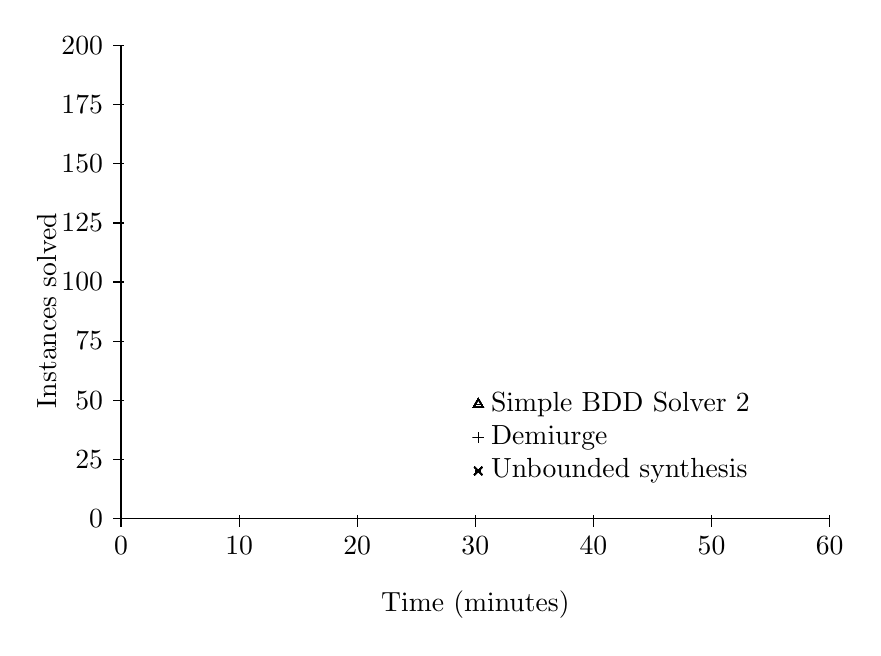
\begin{tikzpicture}[y=0.03cm, x=0.15cm]
        %axis
        \draw (0,0) -- coordinate (x axis mid) (60,0);
            \draw (0,0) -- coordinate (y axis mid) (0,200);
            %ticks
            \foreach \x in {0,10,...,60}
                \draw (\x,1pt) -- (\x,-3pt)
                node[anchor=north] {\x};
            \foreach \y in {0,25,...,200}
                \draw (1pt,\y) -- (-3pt,\y) 
                    node[anchor=east] {\y}; 
        %labels      
        \node[below=0.8cm] at (x axis mid) {Time (minutes)};
        \node[rotate=90, above left=1cm and 0.7cm] at (y axis mid) {Instances solved};
        
        %Plots
        \draw plot[mark=x, mark options={fill=white}] file {bench_termite.dat};
        \draw plot[mark=+, mark options={fill=white}] file {bench_demiurge.dat};
        \draw plot[mark=triangle, mark options={fill=white}] file {bench_simple.dat};

        \begin{scope}[shift={(30,20)}] 
            \draw (0,0) -- 
                plot[mark=x, mark options={fill=white}] (0.25,0) -- (0.5,0) 
                node[right]{Unbounded synthesis};
            \draw[yshift=\baselineskip] (0,0) -- 
                plot[mark=+, mark options={fill=white}] (0.25,0) -- (0.5,0)
                node[right]{Demiurge};
            \draw[yshift=2\baselineskip] (0,0) -- 
                plot[mark=triangle, mark options={fill=white}] (0.25,0) -- (0.5,0)
                node[right]{Simple BDD Solver 2};
        \end{scope}

    \end{tikzpicture}
    \caption{Number of instances solver over time by the unbounded solver, Demiurge,
    and Simple BDD Solver.}\label{fig:cactus}
\end{figure}

Whilst our solver is unable to solve as many instances as other tools, it was
able to solve more unique instances than any solver in the competition. This
confirms that our methodology is able to fill gaps in a state of the art
synthesis toolbox by more efficiently solving instances that are hard for other
techniques. For this reason our solver would be a worthwhile addition to a
portfolio solver. In the parallel track of the competition, \textsc{Demiurge}
uses a suite of 3 separate but communicating solvers. The solvers
relay unsafe states to one another, which is compatible with the set $B^M$ in
our solver. It remains future work to explore the possibility of combining
these solvers.

\section{Related Work}

Synthesis of safety games is a thoroughly explored area of research with most
efforts directed toward solving games with BDDs \cite{burch1990} and abstract
interpretation \cite{walker2014,brenguier2014}. Satisfiability solving has been used
previously for synthesis in a suite of methods proposed by Bloem et al.
\cite{bloem2014}. The authors propose employing competing SAT solvers
to learn clauses, which is similar to our approach but does not unroll the
game. They also suggest QBF solver, template-based, and Effectively
Propositional Logic (EPR) approaches.

SAT-based bounded model checking approaches that unroll the transition relation
have been extended to unbounded by using conflicts in the solver
\cite{mcmillan2002}, or by interpolation \cite{mcmillan2003}. However, there
are no corresponding adaptations to synthesis.

Incremental induction \cite{bradley2011} is another technique for unbounded
model checking with an equivalent synthesis method \cite{morgenstern2013},
which computes sets of states that overapproximate the losing states (similar
to our $B^m$) and another set of winning states (similar to the negation of
$B^M$). Their algorithm maintains a similar invariant over the sets of losing
states as our approach and has the same termination condition. It differs in
how the sets are computed, which it does by inductively proving the number of
game rounds required by the environment to win from the initial state.

There are different approaches to bounded synthesis than the one described
here. The authors of \cite{finkbeiner2013} suggest a methodology directly
inspired by bounded model checking and it has been adapted to symbolic
synthesis \cite{ehlers2010}. Lazy synthesis \cite{finkbeiner2012} is a
counterexample guided approach to bounded synthesis that refines an
implementation for the game instead of an abstraction of it.

The original bounded synthesis algorithm of Narodytska et
al.~\cite{narodytska2014} solves realisability without constructing a strategy.
In \cite{een2015} the realisability algorithm is extended with strategy
extraction. The technique relies on interpolation over abstract game trees to
compute the winning strategy.  In
the present work we use interpolation in a different way in order to learn
losing states of the game.

\section{Conclusion}

We presented an extension to an existing bounded synthesis technique that
promotes it to unbounded safety games. The approach taken as whole differs from
other synthesis techniques by combining counterexample guided game solving with
winning set computation. Intuitively, the abstraction refinement framework of
the bounded synthesis algorithm restricts the search to consider only moves
that may lead to winning strategies. By constructing sets of bad states during
this search we aim to consider only states that are relevant to a winning
strategy while solving the unbounded game.

The results show that our approach is able to solve more unique instances than
other solvers by performing well on certain classes of games that are hard for
other methodologies.

Future work includes incorporating the solver into a parallel suite of
communicating solvers~\cite{bloem2014}. There is evidence that different
solvers perform well on different classes of games. Thus we hypothesise that
the way forward for synthesis tools is to combine the efforts of many different
techniques.

\bibliographystyle{splncs03}
\bibliography{paper}

\end{document}
